In this section, we examine our experimental results to address the above research questions over the performance of our algorithm.

\begin{figure}[t]
 \centering
  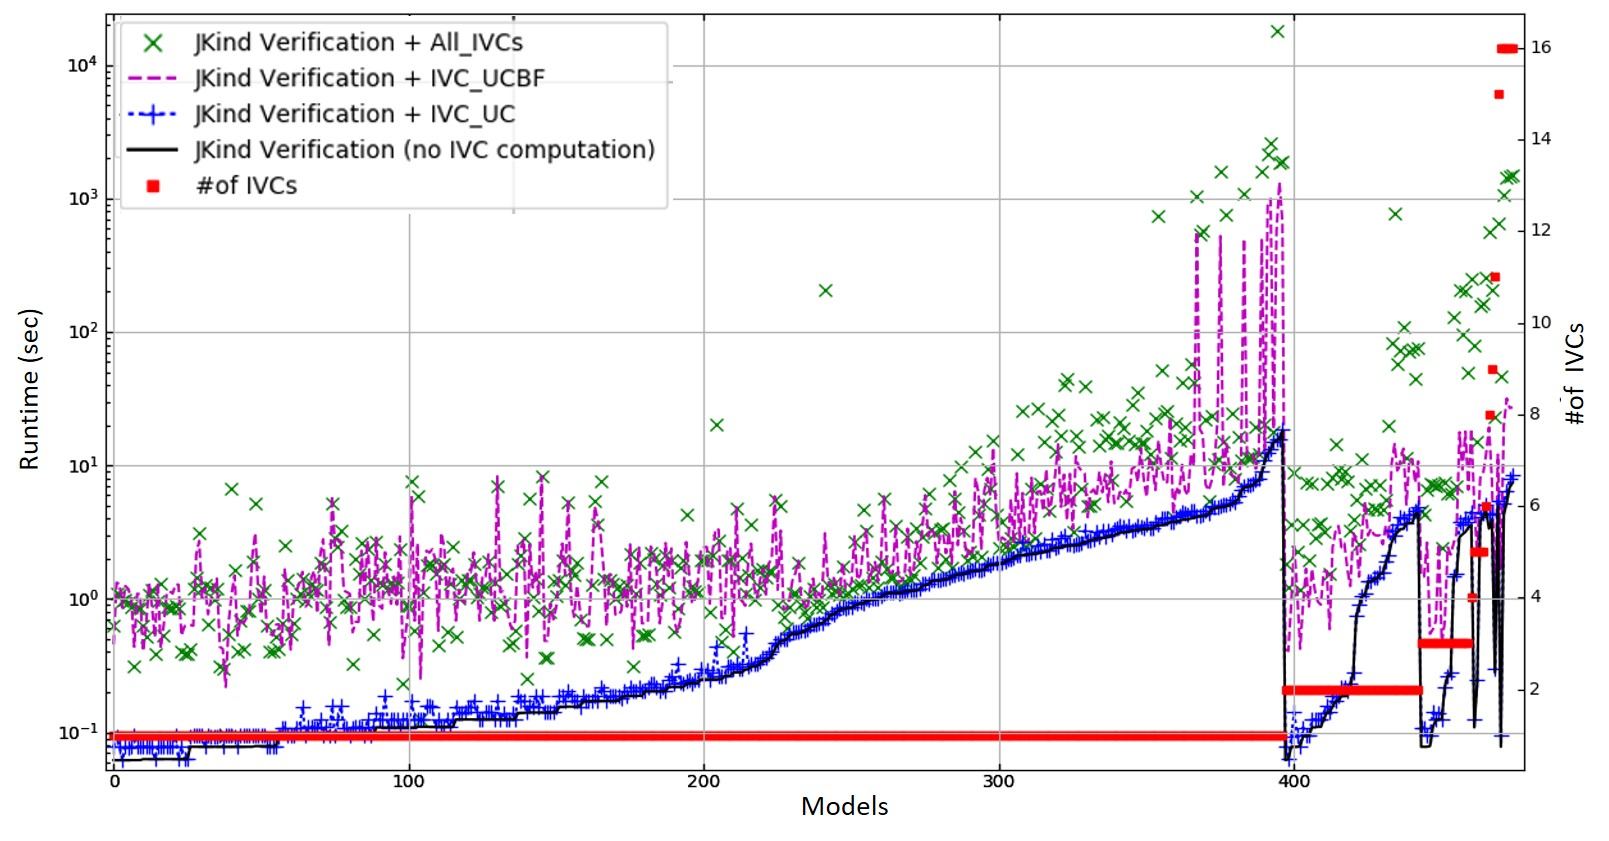
\includegraphics[width=\textwidth]{figs/performance.jpg}
  \label{fig:performance}
  \vspace{-0.2in}
  \caption{Runtime of \aivcalg, \ucbfalg, and \ucalg ~algorithms}
\end{figure}

\textbf{RQ1)} We measured the performance overhead of the algorithms over the time
necessary to find a proof using inductive model checking. Fig. \ref{fig:performance}
 allows a visualization of the  overhead  of the \aivcalg ~algorithm  in  comparison  with \ucalg ~and \ucbfalg. 
 In the figure, the models are ranked along the x-axis by the number of IVCs found by \ucalg ~per model.
 Table \ref{tab:runtime} and Table \ref{tab:overhead} also provide a summary of the computation time and the overhead of different algorithms. 
 As it can be seen, the \ucalg ~algorithm imposes a negligible overhead to the proof time and is quite fast, whereas \ucbfalg ~algorithm adds a substantial penalty in order to find a single IVC. 
 The \aivcalg ~algorithm is able to outperform the \ucbfalg ~in a lot of cases, 
 or perform approximately the same. 
 Note that the \aivcalg ~algorithm could have had better (worse) performance
 if timeout had been set lower (higher).


\begin{table}
  \caption{Runtime of different computations}
   \vspace{-0.1in}
  \centering
  \begin{tabular}{ |c||c|c|c|c| }
    \hline
      runtime (sec)& min & max & mean & stdev \\[0.5ex]
    \hline\hline
    \emph{\small{proof-time}}    & 0.047 & 14.617 & 1.299 & 1.940 \\[0.5ex]
    \aivcalg    & 10.125 & 2375.058& 58.884 & 256.529 \\[0.5ex]
    \ucbfalg &   0.248 & 1323.515 &  17.247& 104.838\\[0.5ex]
    \ucalg&  0.0  & 1.422  & 0.084 & 0.184 \\[0.5ex]
    \hline
  \end{tabular}
  \label{tab:runtime}
\end{table}

\begin{table}
  \caption{Overhead of different algorithms}
   \vspace{-0.1in}
  \centering
  \begin{tabular}{ |c||c|c|c|c| }
    \hline
     algorithm & min & max & mean & stdev \\[0.5ex]

    \hline
    \aivcalg   & 13.642\% & 101034.615\% & 2544.399\% & 7764.159\% \\[0.5ex]
    \ucbfalg &   14.092\% & 111124.432\% &  882.018\% & 1512.071\%\\[0.5ex]
    \ucalg&  0.00\%  & 100.00\%   & 10.226\% & 11.718\% \\[0.5ex]
    \hline
  \end{tabular}
  \label{tab:overhead}
\end{table}

%\takeaway{Computing all minimal Inductive Validity Cores with the \aivcalg ~algorithm is as nearly expensive as computing one single minimal Inductive Validity Core with the \ucbfalg  ~algorithm.
%\ela{Ela: is that fair to say??}}

\textbf{RQ2)} The structure of the model and specification can play a part in how well \aivcalg ~performs. 
Therefore, we would like to examine whether or not there is a relationship between the performance and the size of the model, proof-time, and the diversity of IVCs. A graph showing the size of each model (determined by the number of equations in the model) and the number of IVCs
 along with the running time of \aivcalg ~and normal verification time is shown in Fig \ref{fig:modelsize}. In the figure, the models are ranked along the x-axis by the size of models. The picture shows that as models get larger, 
 
 \begin{figure}[t]
 \centering
  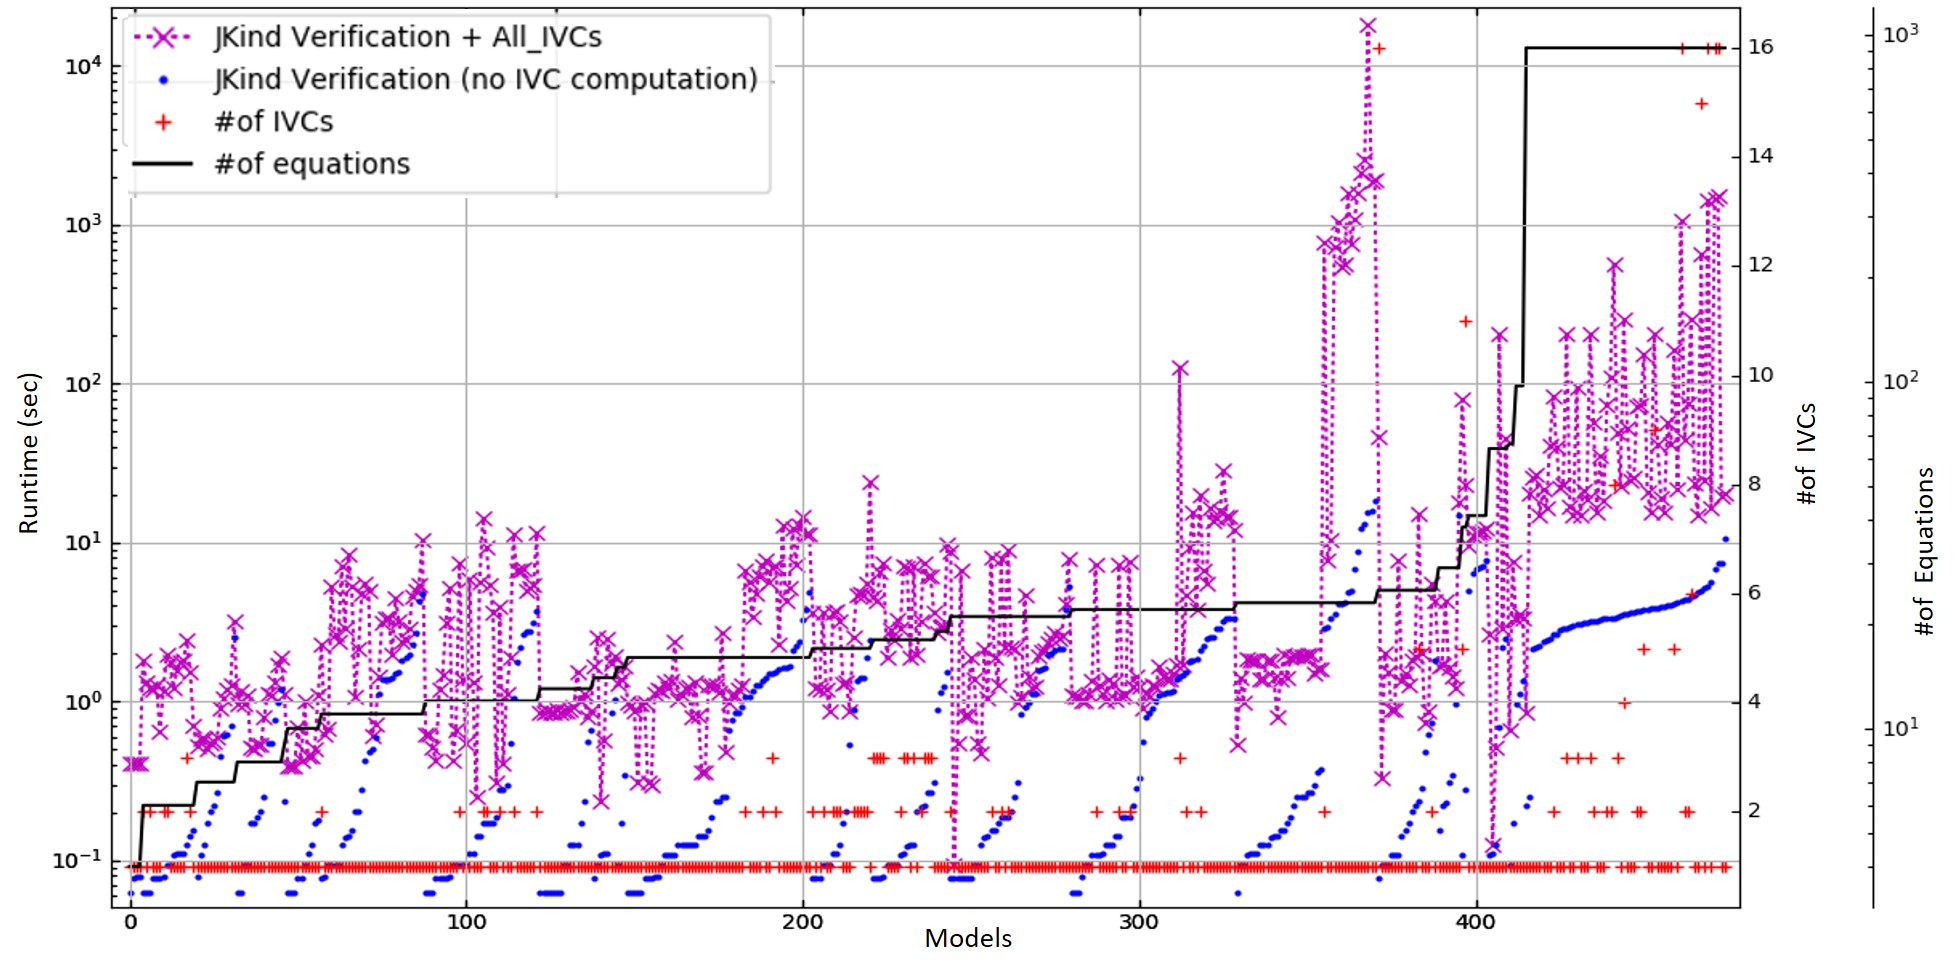
\includegraphics[width=\textwidth]{figs/numofeq.jpg}
  \label{fig:modelsize}
  \vspace{-0.2in}
  \caption{Runtime of \aivcalg along with the model size and number of IVCs}
\end{figure}

\takeaway{} 